%
% fig-kettenzyklen.tex
%
% (c) 2026 Prof Dr Andreas Müller
%
\begin{figure}
\centering
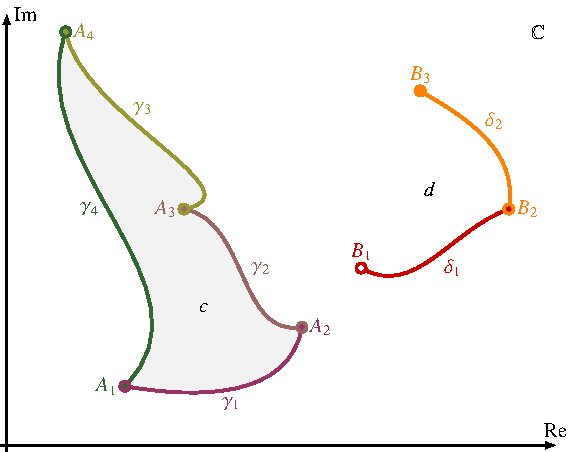
\includegraphics{chapters/030-integration/images/kettenzyklen.pdf}
\caption{Ketten $c=\gamma_1+\gamma_2+\gamma_3+\gamma_4$ und
$d=\delta_1+\delta_2$ sind Linearkombinationen von Wegen.
Der Randoperator extrahiert die Endpunkte mit einem Vorzeichen.
Anfangspunkte sind also offene Kreise, Endpuntke als ausgefüllte
Kreise dargestellt.
Für die Kette $d$ ist $\partial d = B_3-B_1$.
Für die Kette $c$ kommt in $\partial c$ jeder Punkt mit positivem
und negativem Vorzeichen vor, es ist $\partial c=0$.
\label{buch:integration:homologie:fig:kettenzyklen}}
\end{figure}
